\documentclass[11pt]{beamer}
\usetheme{Warsaw}

\definecolor{darkgreen}{RGB}{0,100,0}

\setbeamercolor*{palette primary}{bg=darkgreen, fg = white}
%\setbeamercolor*{palette secondary}{bg=myNewColorB, fg = green}
%\setbeamercolor*{palette tertiary}{bg=myNewColorC, fg = green}
%\setbeamercolor*{palette quaternary}{bg=myNewColorD, fg = green}


\usepackage[utf8]{inputenc}
\usepackage[english]{babel}
\usepackage{amsmath}
\usepackage{amsfonts}
\usepackage{amssymb}
\usepackage{graphicx}
\author{ Samuel \textsc{ORTION} }
\title{ AlgoR.dijkstra - On Graph Shortest Path }
\setbeamercovered{transparent} 
\setbeamertemplate{navigation symbols}{} 
\logo{
\includegraphics[width=0.15\textwidth]{./media/univ-evry.fr-logo.noir.png}} 
\institute{ Université d'Évry val d'Essone - Paris-Saclay } 
\date{ 2022 }
\subject{ Computer Science } 

\begin{document}

\begin{frame}
\titlepage
\end{frame}

\begin{frame}
\tableofcontents
\end{frame}

\section{Introduction}

\subsection{What is this?}

\begin{frame}{AlgoR}

AlgoR is a set of R Packages to learn algorithmic and RCpp programming.

\textbf{Subject} : see \href{https://github.com/vrunge/TSP/blob/main/simulations/projetsM2_Algorithmique_2022_2023.pdf}{V. RUNGE projet statement (fr.)}

\textbf{AlgoR.dijkstra} : the \href{https://github.com/UncleSamulus/AlgoR.dijkstra}{R package} that implements shortest path algorithm.

\end{frame}

\section{The Dijkstra Algorithm}

\subsection{But what is a graph?}

\begin{frame}{Graph}
	Let $G = (V, E)$ be a graph, where $V$ is a set of vertices and $E$ is a set of edges. \\
	An edge $e = (u, v)$ is a pair of vertices $u$ and $v$ such that $u, v \in V$. \\

	\begin{itemize}
		\item $G$ is a directed graph if $e = (u, v)$ implies $u \rightarrow v$.
		\item $G$ is an undirected graph if $e = (u, v)$ implies $u \leftrightarrow v$.
	\end{itemize}

	We can add a weight $w$ to each edge $e = (u, v)$, to get a weighted graph. \\
\end{frame}

\begin{frame}{Directed graph}

\begin{figure}[h]
	\centering
	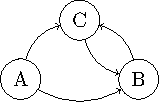
\includegraphics[width=0.5\textwidth]{./content/figures/directed_graph.pdf}
	\caption{Directed graph}

	\begin{math}
		G = (V, E) = \left( \{A, B, C\}, \{(A, B), (A, C), (B, C), (C, B)\} \right)
	\end{math}
\end{figure}

\end{frame}
\begin{frame}{Weighted graph}
	\begin{figure}
\end{figure}
\begin{figure}
	\centering
	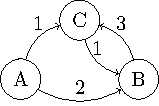
\includegraphics[width=0.5\textwidth]{./content/figures/weighted_graph.pdf}
	\caption{Weighted directed graph}
\end{figure}

\begin{math}
	G = (V, E) = \left( \{A, B, C\}, \{(A, B), (A, C), (B, C), (C, B)\} \right)
	\newline
	W = \{2, 1, 3, 1\}
\end{math}
\end{frame}

\subsection{The Problem...}

\begin{frame}{Shortest Path}
	Let be a graph $G$, a source vertex $s$ and a destination vertex $d$. \\
	What is the \textbf{shortest path} from $s$ to $d$? \\
	(That is to say the set of vertex $S$ such that there exists an edge between each vertex in $S$ and the next one in $S$ and the sum of the weight of the edges is minimal.)
\end{frame}

\begin{frame}{Shortest Path - An example}

\begin{figure}
	\centering
	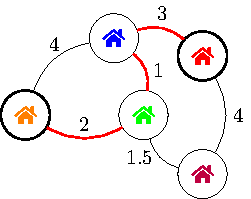
\includegraphics[width=0.5\textwidth]{./content/figures/weightedgraph_city_example.pdf}
	\caption{Find the shortest path from the orange house to the red house}

\end{figure}
\end{frame}

\end{document}
